\section{Project Specifications} \label{sec:spec}

The goal of this project is to gain insights of deep reinforcement learning as a means of implementing both algorithm and simulation environment,  training policies, and evaluating their performance \cite{ref:spec-report}. The engineering part of this project mainly consists of implementing the algorithm and environment, as well as training the policies. Therefore, this is a research-oriented pure software engineering project.

For this project, mapless navigation was chosen as the study case of deep reinforcement learning. From the perspective of deep reinforcement learning, any task that it can solve is nothing more than a dataset described by a Markov decision process. Therefore, any task that can be formulated as a Markov decision process is a potential candidate for this project. Initially, quadrupedal locomotion learning was considered, but due to its high engineering complexity, which is close to the level of doctoral research, the idea was eventually abandoned in favor of mapless navigation on account of time constraints.

Mapless navigation is a robotic task that requires the robot's motion planner to navigate the robot to a target location without relying on a map, while avoiding obstacles along the way. In the framework of deep reinforcement learning, the motion planner here can be simply modelled by a policy neural network. The performance of the motion planner can be gradually improved by updating its model weights according to a predefined reward signal through training using reinforcement learning algorithms.

The main line of this project is planned step by step. First, familiarise with the algorithms by literature reading. Next, implement them and group them as a software package. Then, develop a simulation training environment for mapless navigation. Finally, combine the algorithms with the environment to train policies and gradually increase the complexity of the environment depending on the performance at each stage. The focus is on gaining a deeper understanding of reinforcement learning through the above process. The goal is divided into three specific objectives:
\begin{enumerate}[label=\arabic*), nosep, leftmargin=*]
    \item Implement deep reinforcement learning algorithms and a simulated mapless navigation training environment.
    \item Training policies to move towards a target on a level ground with no obstacles.
    \item Policy training for the case with obstacles.
\end{enumerate}
Tasks and deliverables encompass both research and engineering efforts. They are detailed below which will satisfy the objectives set out. The verification metrics are given in the Table \ref{table:specifications-verification-matrix}.

\begin{enumerate}[label=Task \arabic*{,}, leftmargin=*]
    \item \textbf{Literature Survey}: This task will review the recent work on mapless navigation that use deep reinforcement learning. The outcome will be a brief report on the topic (D.1).
    \item \textbf{Library Implementation}: State-of-the-art deep reinforcement learning algorithms, including DDPG, TD3, and SAC, will be implemented and grouped together as a Python package (D.2).
    \item \textbf{Training Environment Implementation}: An flat floor indoor environment will be implemented in the Gazebo Classic simulator. The environment can be completely obstacle-free, may contain some fixed obstacles, or may include randomly moving obstacles, depending on the performance of the training at each stage to gradually increase the complexity of the environment (D.3).
    \item \textbf{Trained Near-optimal Policies}: The policies will be trained by using the D.2 and D.3 until they reach their near-optimal point (the episodic return stops increasing). The performance of the near-optimal policies will be illustrated by episodic return curves and visualised in demonstration videos and a rendering program (D.4).
    \item \textbf{Insights}: The research outcomes will be reported in the project final report (D.5).
\end{enumerate}

\begin{enumerate}[label=D. \arabic*:, leftmargin=*]
    \item Brief report on the recent work on mapless navigation using deep reinforcement learning.
    \item A library implementation.
    \item A training environment implementation.
    \item Trained policies with illustration and visualisation of their performance.
    \item Report the insights on deep reinforcement learning gained through experience.
\end{enumerate}

\begin{table}[htbp]
   \centering
   \caption{Specifications verification metrics \cite{ref:spec-report}}
   \label{table:specifications-verification-matrix}
   \begin{tblr}{
      width=0.9\linewidth,
      colspec={|X|X|},
      hlines,
   }
   Specification & Verification \\
   \hline
   Implement state-of-the-art deep reinforcement learning algorithms. & Test on baseline environments. \\
   Train policies in an empty world. & Robot can reach the target position. \\
   Train policies in an indoor environment filled with obstacles. & Robot can reach the target position and not collide with obstacles. \\
   \end{tblr}
\end{table}

The project is expected to take seven months to complete. To ensure the success of this project, a timeline has been established to keep track of the progress of each task. The timeline includes specific milestones and deadlines for each task, as well as regular meetings to discuss the progress and make any necessary adjustments. The timeline is parially represented as a Gannt chart. Below is the original Gannt chart:

\begin{figure}[htbp]
   \centerline{
   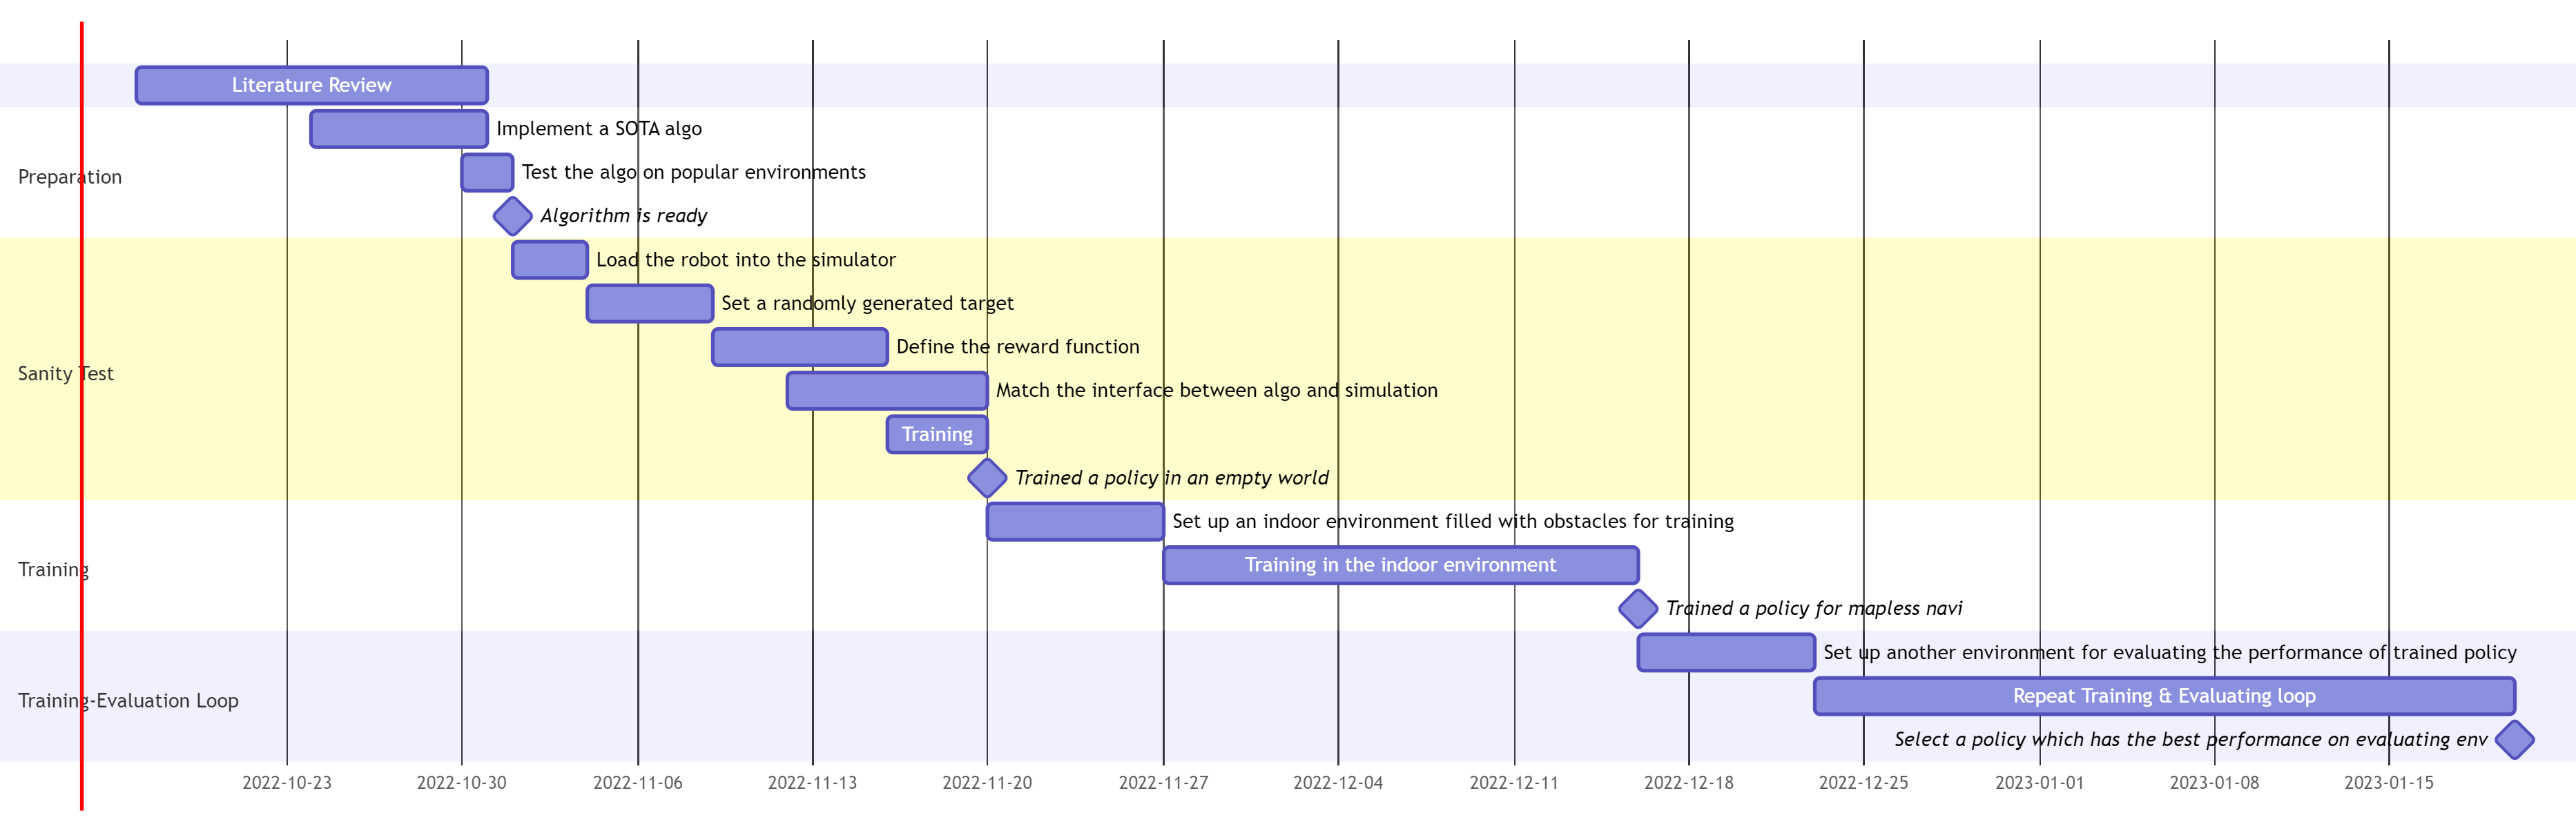
\includegraphics[width=\paperwidth]{gantt}}
   \caption{Original plan \cite{ref:spec-report}}
   \label{fig:gantt}
\end{figure}

\newpage